\documentclass[11pt]{article}

\usepackage{exscale}
\usepackage{graphicx}
\usepackage{amsmath}
\usepackage{latexsym}
\usepackage{times,mathptm}
\usepackage{epsfig}
\usepackage{setspace}

\textwidth 6.5truein          
\textheight 9.0truein
\oddsidemargin 0.0in
\topmargin -0.6in

\parindent 0pt          
\parskip 5pt
\def\baselinestretch{1.1}

\begin{document}

\begin{LARGE}
\centerline {\bf CSci 423 Homework 5}
\end{LARGE}
\vskip 0.25cm

\centerline{Due: 1:00 pm, Wednesday, 10/17}
\centerline{Eric Shih}

\begin{enumerate}
  \item (10 points) Exercise 2.6 (b) and (d) on page 129.
    \begin{description}
     \item{b.} \\
	  $S \to aSb |Ra|bR$ \\
	  $R \to Ra|Rb|\epsilon $
     \item{d.} \\
	  $S \to T|U\#T|T\#U|U\#T\#U$ \\
	  $T \to a|b|aTa|bTb|\#|\#U\#|\epsilon$ \\
	  $U \to U\#W|W$ \\
	  $W \to aW|bW|\epsilon$
    \end{description}

  \item (5 points) Exercise 2.9 on page 129. 
    \begin{description}
     \item CFG: \\
      $S \to R|T $ \\
      $R \to aRbU|\epsilon $ \\
      $T \to WbTc|\epsilon $ \\
      $U \to cU|\epsilon $ \\
      $W \to aW|\epsilon $
     \item Yes the grammar is abiguous because there is a string a string that can be derived in more than 1 fashion.
	   abc can be derived: \\
	   1) $S \implies R \implies aRbU \implies abU \implies abc$ \\
	   2) $S \implies T \implies WbTc \implies Wbc \implies abc$
    \end{description}


  \item (10 points) Exercise 2.13 on page 129.\\
    *Referenced: http://courses.engr.illinois.edu/cs373/fa2010/Problem Sets/hw9sol.pdf * \\
    a) {\bf Description:} The resulting string of L(G) can result in two situations. One will have one \# in between zero or more 0s, 
    where the 0s on the right of the \# is twice the number of 0s on the left. The situation results in a string
    that will have two \#'s with any number of 0s within the string. \\ 
    b) {\bf Proof:} We will use the closure property
    \begin{description}
     \item Consider a homomorphism $h_1$: ${0,1} \to {0,\#}$, such that $h_1(0) = 0, 
	   h_1(\#) = \#, and  h_1(1) = 00$. Let $K_1 = h_{1}^{-1} (L(G))$.
     \item Let $K_2 = K_1 \cap L(0^i \# 1^i)$. Observe that the only strings
	   in L(G) that have a single \# symbol are those belonging to $L_2$, and given
	   the definition of homomorphism $h_1$, we can conclude that $K_2 = {0^i \# 1^i 
	   i \geq 0 }$.
     \item Consider the homomorphism $h_2 : {0,1, \#} \to {0,1}$, where $h_2$(0) = 0, 
	   $h_2$(1) = 1, and $h_2$(\#) = $\epsilon$. Observe that $K_3 = h_2(K_2) = 
	   {0^n1^n|n \geq 0}$. 
    \end{description}
    Since $K_1,K_2,K_3$ are obtained from L(G) through regularity preserving operations
    and $K_3$ is non-regular, we can conclude that L(G) is not regular.

  \item (5 points) Exercise 2.14 on page 129.
    \begin{description}
     \item{1.} $S_0 \to A$ \\
	   $A$ $\to BAB | B | \epsilon$ \\
	   $B \to 00 | \epsilon$
     \item{2.} $S_0 \to A$ \\
	   $A$ $\to BAB | B | AB | BA | \epsilon$ \\
	   $B \to 00$
     \item{3.} $S_0 \to A | \epsilon$ \\
	   $A$ $\to BAB | B | AB | BA | BB$ \\
	   $B \to 00$
     \item{4.} $S_0 \to BAB | B | AB | BA | BB | \epsilon$ \\
	   $A$ $\to BAB | B | AB | BA | BB$ \\
	   $B \to 00$
     \item{5.} $S_0 \to UB | 0C | AB | BA | BB | \epsilon$ \\
	   $A$ $\to UB | 0C | AB | BA | BB $ \\
	   $B \to 0C$ \\
	   $C \to 0 $\\
	   $U \to BA$
    \end{description}

  \item (10 points) Exercise 2.10 on page 129. (Give the state diagram of your PDA.) \\
    {\bf Description:} The PDA checks the case that $i = j$ and in another part that $j = k$. The first part has
    an $a$ pushed for every $a$ read, and an $a$ popped for every $b$ read. $\$$ will be the only one in
    the stack if there is an equal number of a's and b's. c's are then read and dealt with at the finish state.
    In the second part, a's are read and produce nothing, while a $b$ will be pushed for every $b$ read, and popped
    off for every $c$ read. \\
    {\bf State Diagram:}
    \begin{center}
      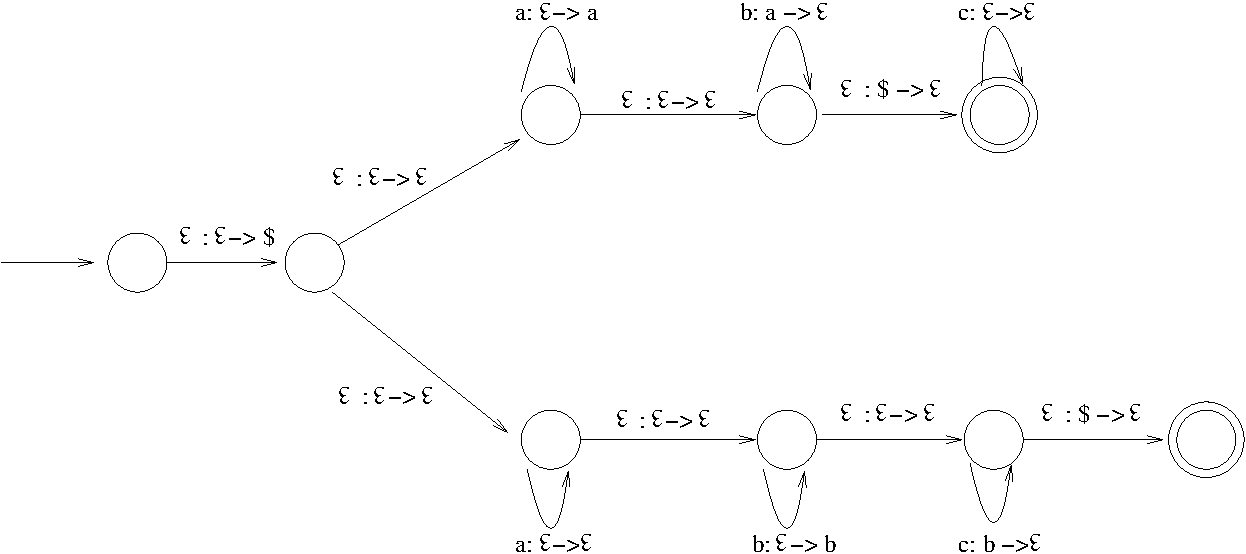
\includegraphics[scale=.7] {fig1.pdf}
    \end{center}
\end{enumerate}

\end{document}